\documentclass[10pt,norsk,a4paper]{article}
\usepackage[utf8]{inputenc}
\usepackage[T1]{fontenc}
\usepackage[norsk]{babel}
% - PDF-relatert
\usepackage{hyperref,pdfpages,hypcap}
\hypersetup{colorlinks=true,allcolors=.}
\newcommand\fhref[2]{%
	\href{#1}{#2}\footnote{\url{#1}}%
}
% Andre pakker
\usepackage[cm]{fullpage}
\usepackage{parskip,multicol,textcomp,amssymb,graphicx,color,enumitem}
% - Korreksjon av fotnoter i seksjoner/overskrifter
\usepackage[stable]{footmisc}
% - Skrifttype
\usepackage[bitstream-charter]{mathdesign}
% - Kommentarer
\usepackage{comment}


\title{Generalforsamling \\
	Våren 2019\\[3cm]
	
\includegraphics[width=0.5\textwidth]{cyb-logo.eps}\\[-.5cm]}
\date{23.\ mai 2019}
\author{Cybernetisk Selskab}

% Blank header, samt footer med side x av y
\usepackage{fancyhdr}
\pagestyle{fancy}
\renewcommand{\headrulewidth}{0pt}
\fancyhead{}
\cfoot{Side~\thepage\ av~\pageref*{lastpage}}


\begin{document}

\maketitle{}
\newpage
\tableofcontents

\part*{Agenda}

\section{Valg av møteleder}

\section{Valg av referent}

\section{Valg av protokollunderskrivere}

\section{Valg av tellekorps}

\section{Godkjenning av innkalling}

\section{Godkjenning av dagsorden}

%\newpage

\section{Semesterberetninger}
\subsection{Semesterberetning ved leder}

Thor has to do this right here!

\subsection{Semesterberetning ved kjellermogul}

Go Go Kjellermogul!


%\newpage

\section{Kasserer orienterer}
\subsection{Regnskapets tilstand}
Kasserer presenterer regnskapet.

\subsection{Revidert budsjett for våren 2019}
Kasserer presenterer budsjett.

\subsection{Foreløpig regnskap for høsten 2018}
Kasserer presenterer foreløpig regnskap.

\section{Kontigentfastsettelse}
Hovedstyret foreslår å holde medlemskontigenten på kr.~40,-.

\newpage

\section{Valg}

\begin{minipage}[t]{0.49\textwidth}
\subsection{Hovedstyret}
Man velges inn i hovedstyret for ett år av gangen.

\subsubsection{Leder}
\subsubsection{Nestleder}
\subsubsection{Arrangementssjef}
\subsubsection{Rekrutteringsansvarlig}
\subsubsection{Internansvarlig}

\end{minipage}
\begin{minipage}[t]{0.49\textwidth}
\subsection{Kjellerstyret} %TODO Oppdater listen med verv
Alle verv som er til valg i kjellerstyret gjelder for ett semester av gangen. Med unntak av Økonomiansvarlig som blir valgt inn for to semester.

\subsubsection{Innkjøpsansvarlig}
\subsubsection{Barsjef}
\subsubsection{Kafésjef}
\subsubsection{Teknisk ansvarlig}
\subsubsection{DJ-sjef}
\subsubsection{Utlånsansvarlig}
\subsubsection{Arrangementskoordinator}

\newpage

\section{Vedtektsforslag}

\subsection{Personlig oppmøte eller mulighet for fullmakt}
\subsubsection{Alt. 1: personlig oppmøte kreves for å kunne avgi enhver stemme:
               nytt punkt under §7 eller tillegg til punkt §7g}

Forslaget eliminerer muligheten for å avgi fullmakt til en annen person for å stemme.

\subsubsubsection{Nytt punkt under: §7}
\begin{quote}
	\begin{enumerate}
		\item[§7k] Man må være personlig oppmøtt på generalformalingen for å kunne avgi stemme
	\end{enumerate}
\end{quote}

\subsubsubsection{Pålegg: §7g}
\begin{quote}
    \begin{enumerate}
        \item[§7g] Stemmerett har alle som er medlem, jf. §2, minst én uke før generalforsamling,
                  \textcolor{red}{og har møtt opp personlig på  generalforsamling}.
    \end{enumerate}
\end{quote}

Hovedstyret støtter ikke forslaget


\subsubsection{Alt. 2: opptil én fullmakt kan avgis per person: to nye punkter under §7}

Forslaget fastsetter muligheten og kravene for å avgi stemmer via fullmakt,
og begrenser det til én fullmakt per hver stemmeberettigede til stede.

Åpne for at hver oppmøtte kan maksimalt ha en fullmakt fra en annen person.
Dette gjør at hvis man faktisk har en grunn til å ikke komme er det enda mulig å fikse med noe.

\subsubsubsection{Nytt punkt: §7k}
\begin{quote}
    \begin{enumerate}
        \item[§7k]
            Hver stemmeberettigede tilstede på generalforsamling kan stille med
            stemmefullmakt for én annen  stemmeberettig.

            Fullmakten må inneholde følgene punkter:
            \begin{itemize}
                \item Navn på hvem fullmakten er gitt til
                \item Navn på den som gir fullmakten
                \item Dato for generalforsamling
                \item Signaturer fra begge parter involvert.
            \end{itemize}
    \end{enumerate}
\end{quote}

Enda ett punkt som kan følge hvis punkt over går gjennom:

\subsubsubsection{Nytt punkt under: §7l}
\begin{quote}
    \begin{enumerate}
        \item[§7l] Fullmakter gjelder kun ved vedtektsaker og ikke valg av styremedlemmer
    \end{enumerate}
\end{quote}

Hovedstyret støtter §7k, og støtter ikke §7l.

\end{minipage}

\newpage

\section{Utdeling av pins}

Arkivar deler ut pins.


\part*{Vedlegg}\label{lastpage}
\addcontentsline{toc}{part}{Vedlegg}

\newpage
\phantomsection{}
\addcontentsline{toc}{section}{Vedtekter for Cybernetisk Selskab} % chktex
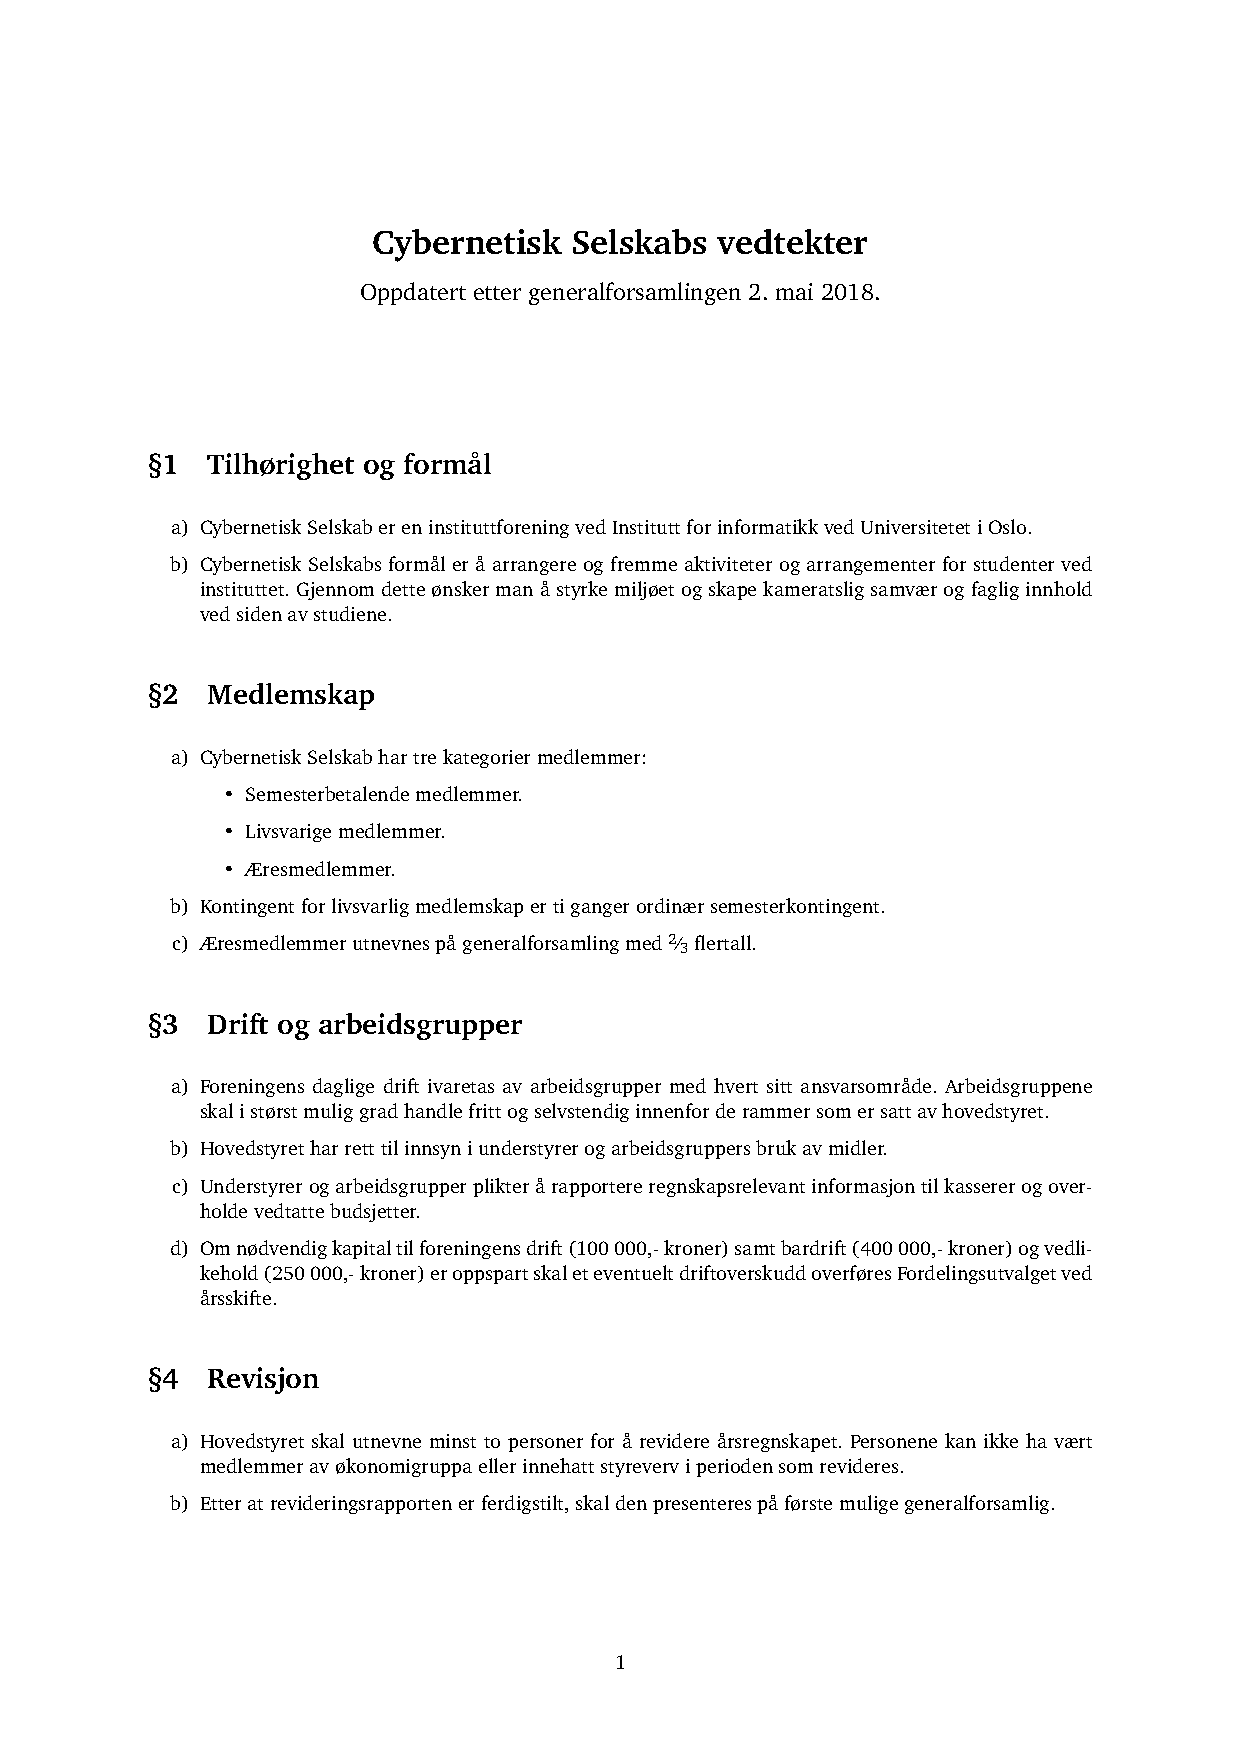
\includepdf[pages=-]{../vedtekter/vedtekter.pdf}

\end{document}
